\begin{figure}[t]
    \centering
    \begin{subfigure}[t]{\textwidth}
        \centering
        \captionsetup{justification=centering}
        
\includegraphics[width=0.57\textwidth]{figs/scaling_laws/scaling_laws_label.pdf}
    \end{subfigure}
    \centering
    \begin{subfigure}[t]{0.265\textwidth}
    \captionsetup{justification=centering}
        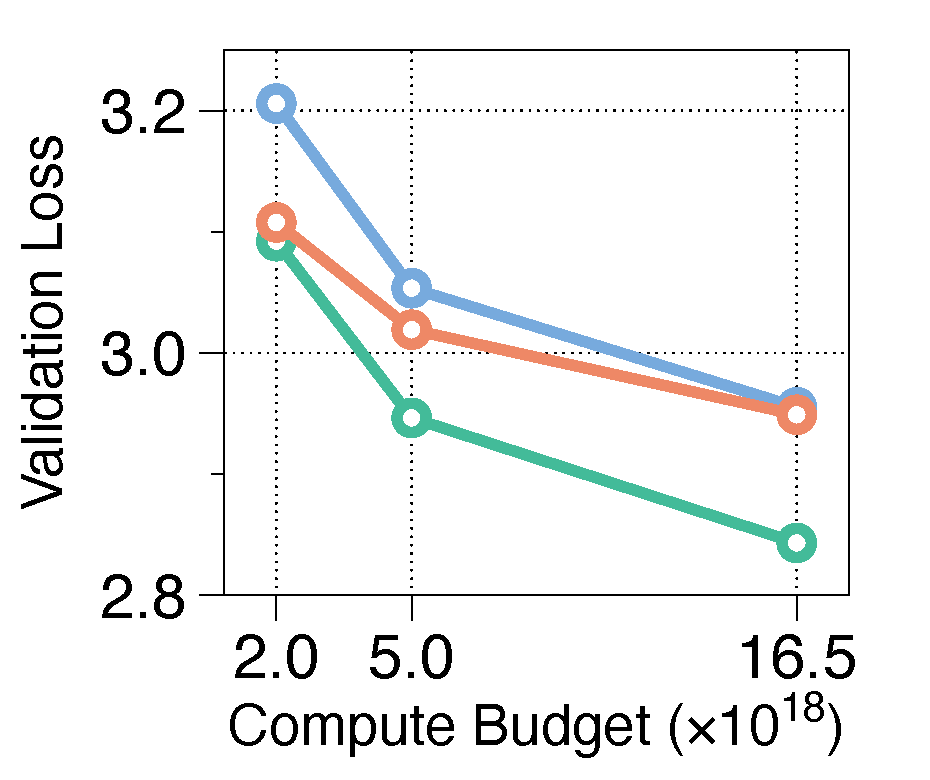
\includegraphics[width=\textwidth]{figs/scaling_laws/135M_base.pdf}
        \subcaption{135M-based model}
    \end{subfigure}
    \hspace{-8pt}
    \centering
    \begin{subfigure}[t]{0.24\textwidth}
    \captionsetup{justification=centering}
        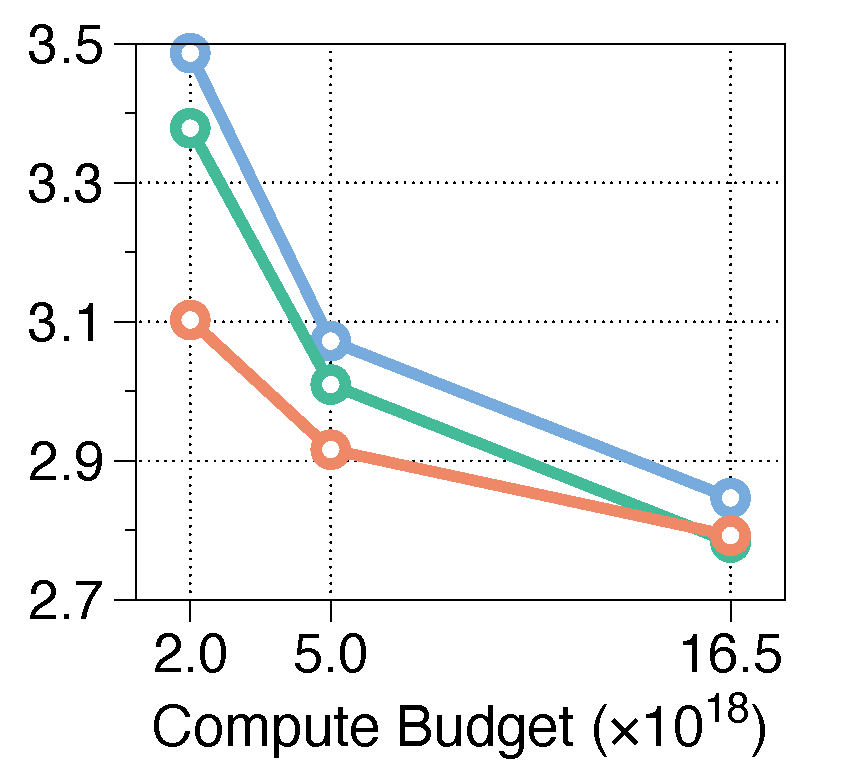
\includegraphics[width=\textwidth]{figs/scaling_laws/360M_base.pdf}
        \subcaption{360M-based model}
    \end{subfigure}
    \hspace{-8pt}
    \centering
    \begin{subfigure}[t]{0.24\textwidth}
    \captionsetup{justification=centering}
        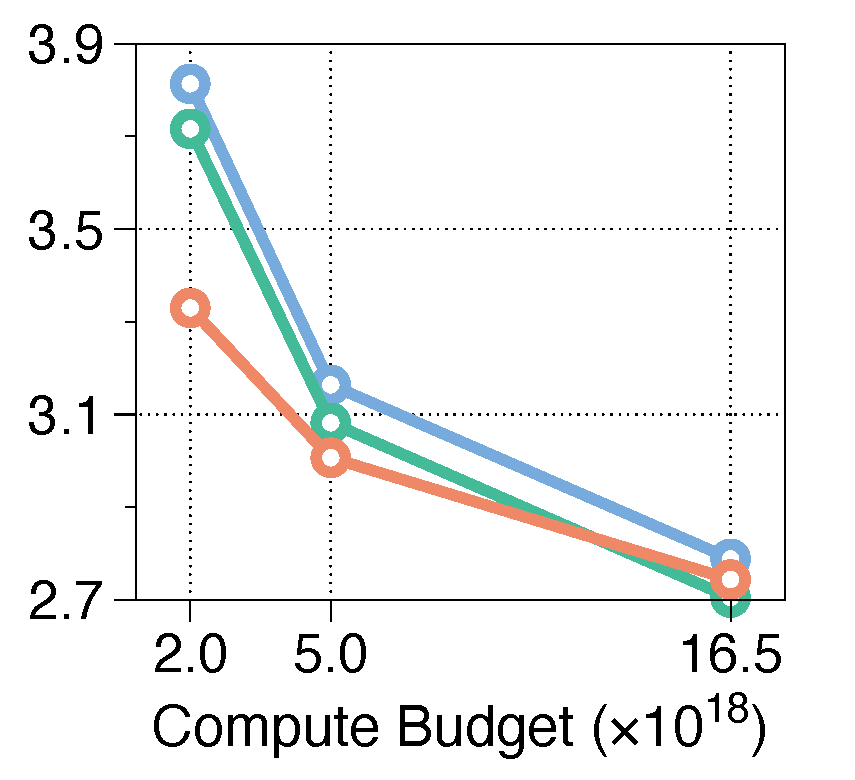
\includegraphics[width=\textwidth]{figs/scaling_laws/800M_base.pdf}
        \subcaption{730M-based model}
    \end{subfigure}
    \hspace{-8pt}
    \centering
    \begin{subfigure}[t]{0.24\textwidth}
    \captionsetup{justification=centering}
        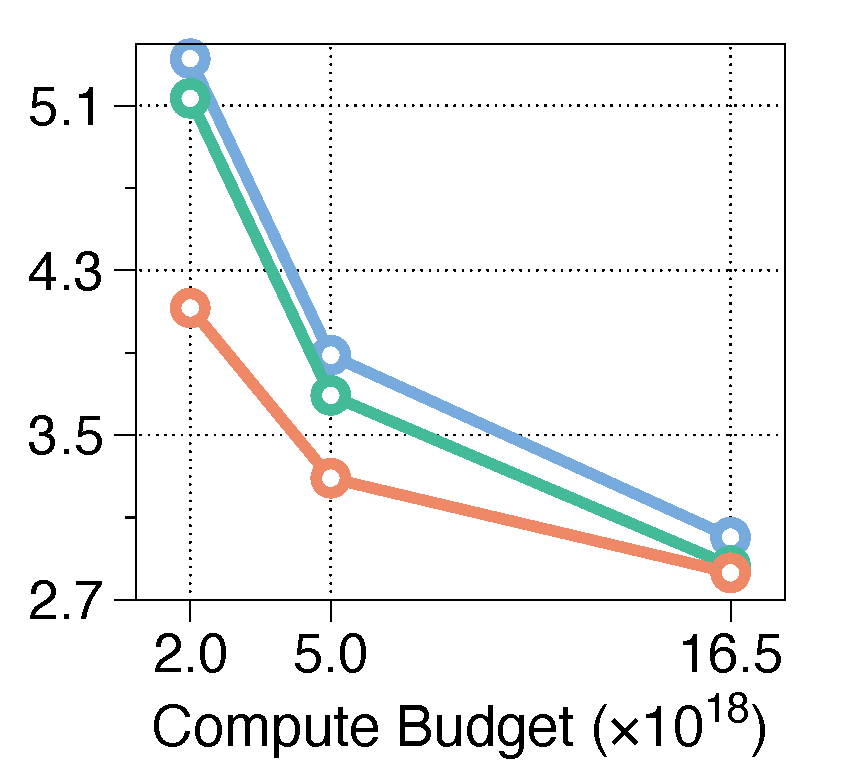
\includegraphics[width=\textwidth]{figs/scaling_laws/1.7b_base.pdf}
        \subcaption{1.7B-based model}
    \end{subfigure}
    \caption{
    Validation loss across different compute budgets across four model sizes: 135M, 360M, 730M, and 1.7B parameters. For MoR models, we use expert-choice routing and recursion-wise caching. MoR consistently outperforms recursive baselines and matches or exceeds the standard Transformers at larger scales, despite using significantly fewer parameters (approximately one-third due to layer tying with $N_R=3$).\looseness=-1
    }
    \label{fig:scaling_laws_app}
\end{figure}
